\documentclass[letterpaper]{article}
\usepackage[paperwidth=8.5in,paperheight=11in,margin=0in]{geometry}
\usepackage{tikz}
\usetikzlibrary{arrows.meta}
\pagestyle{empty}

\begin{document}
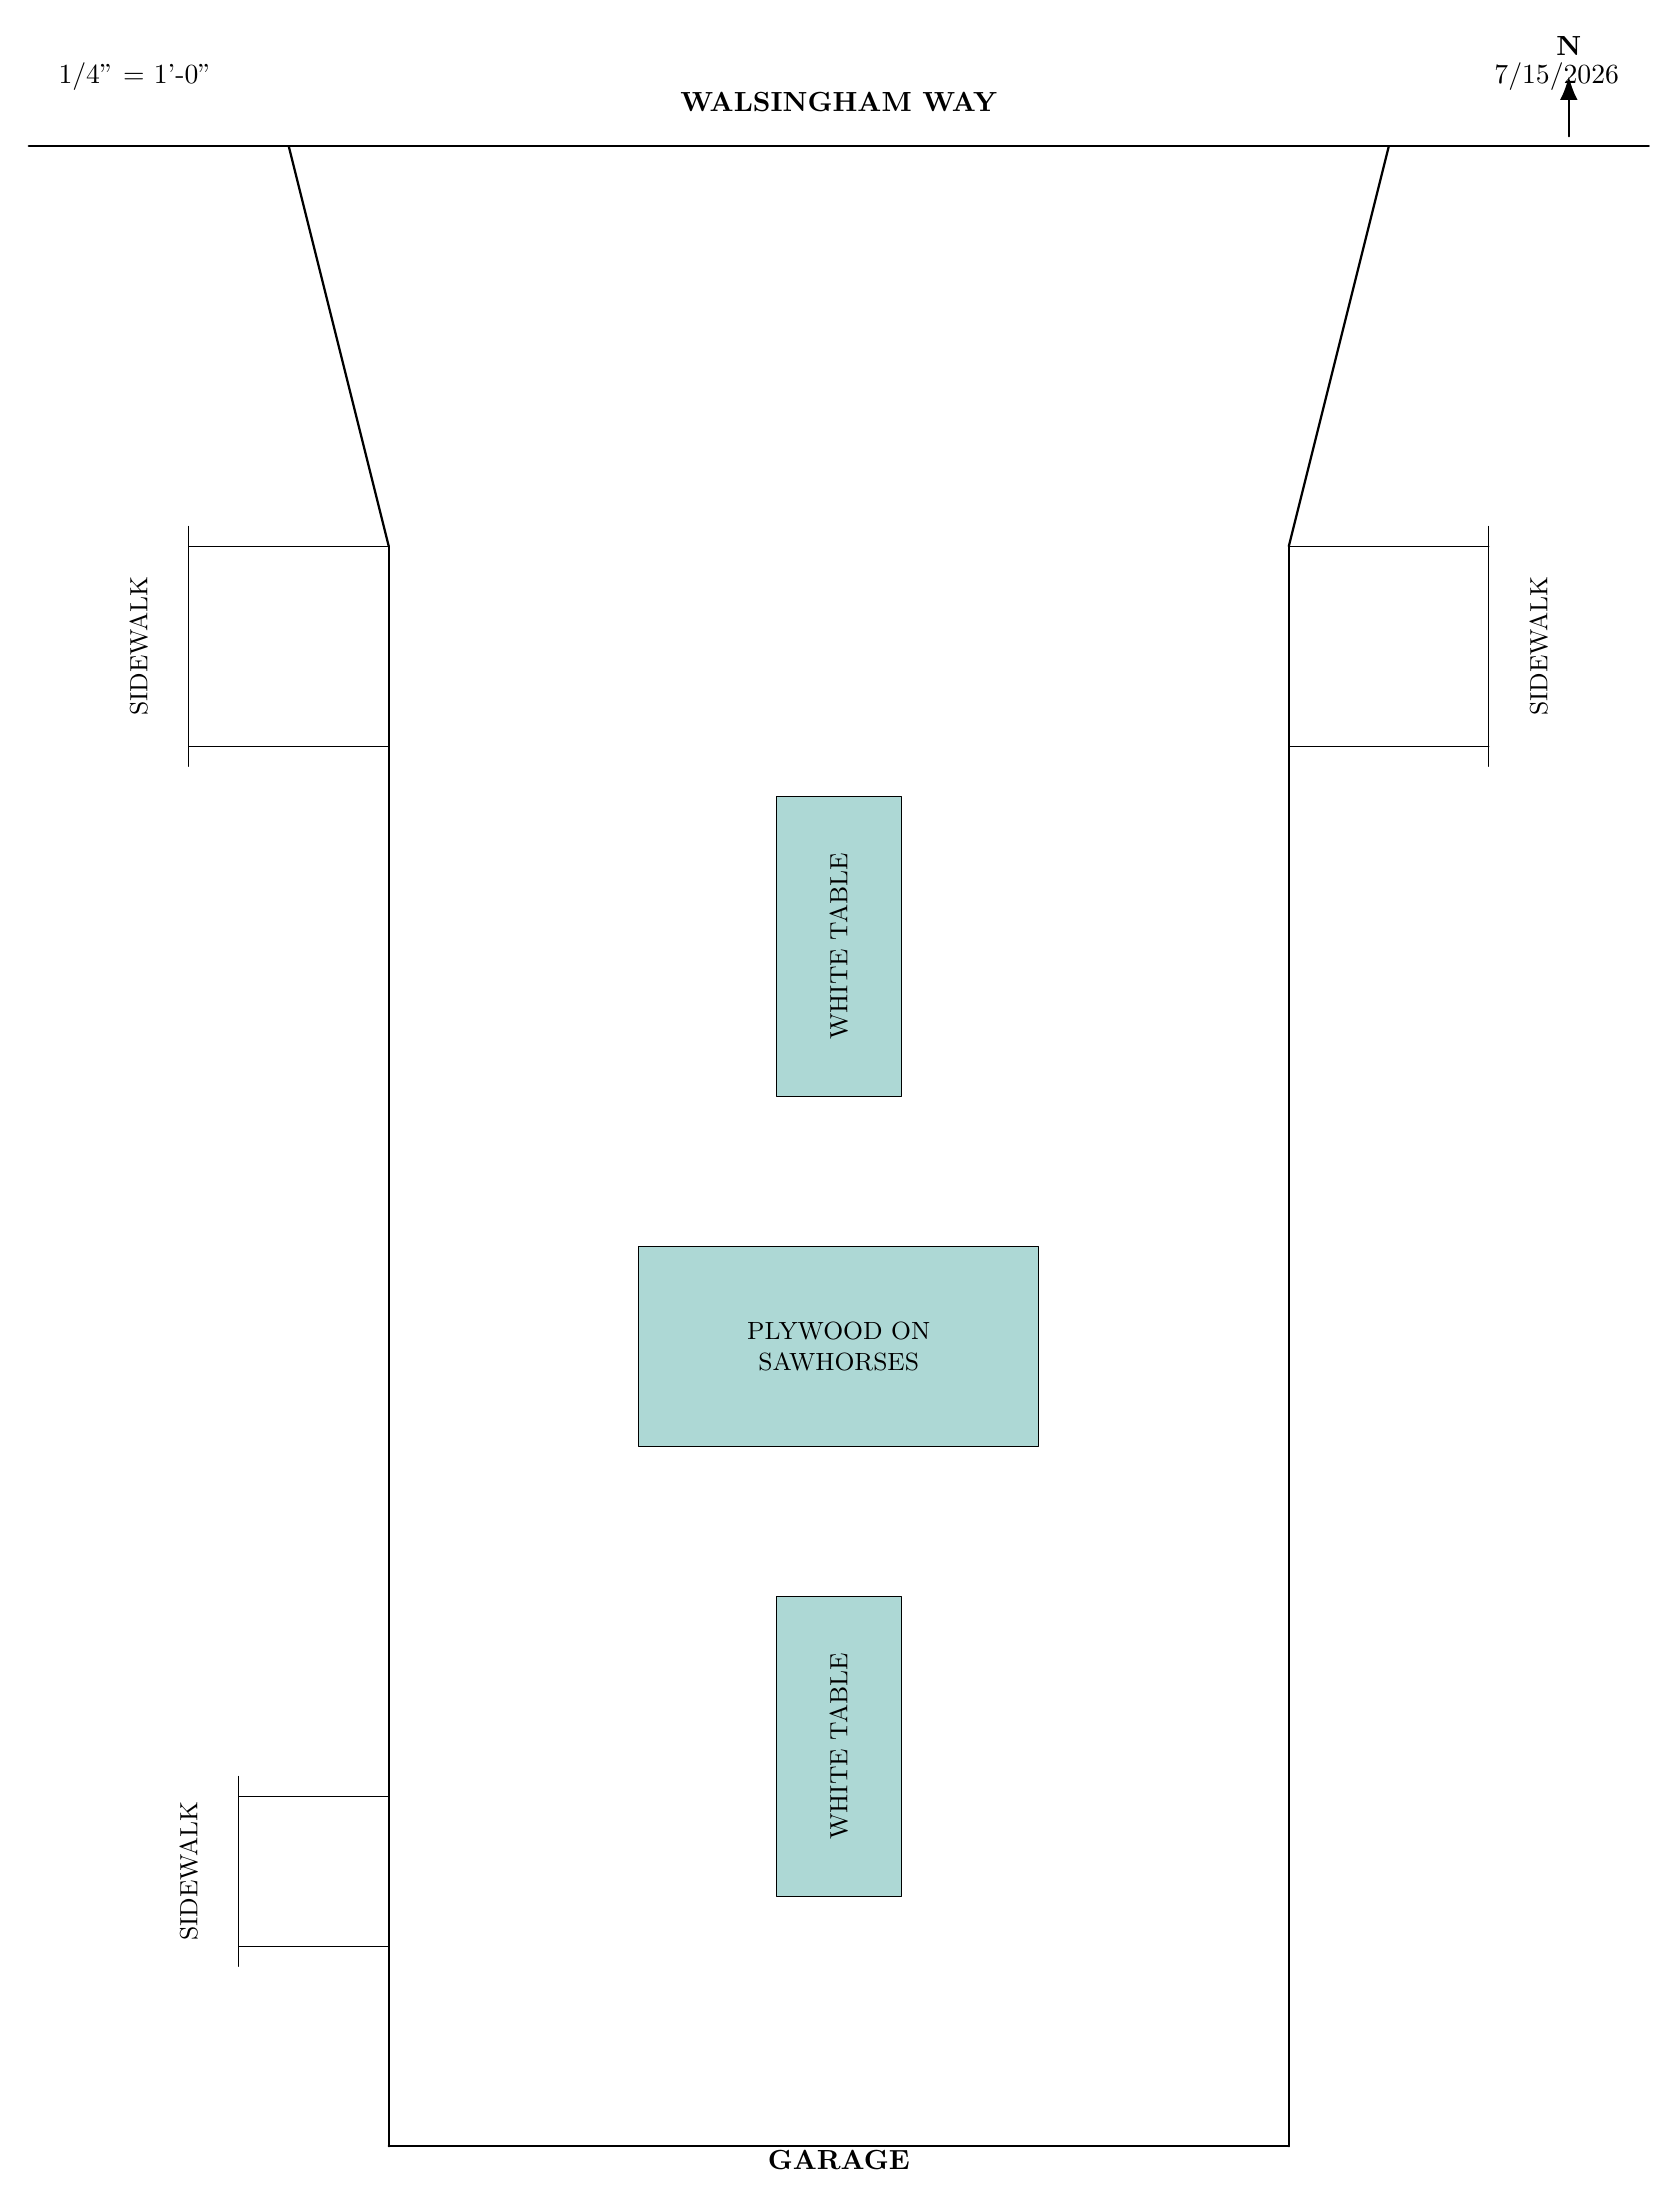
\begin{tikzpicture}[x=1in,y=1in,line join=round,line cap=round]

  % ---- street ----
  \draw[thick] (0.2,10.4) -- (8.3,10.4);
  \node[font=\bfseries] at (4.25,10.620000000000001) {WALSINGHAM WAY};

  % ---- driveway verticals + flares ----
  \draw[thick] (2.0,0.4) -- (2.0,8.4);
  \draw[thick] (6.5,0.4) -- (6.5,8.4);
  \draw[thick] (2.0,8.4) -- (1.5,10.4);
  \draw[thick] (6.5,8.4) -- (7.0,10.4);

  % ---- garage line ----
  \draw[thick] (2.0,0.4) -- (6.5,0.4);
  \node[font=\bfseries] at (4.25,0.33) {GARAGE};

  % ---- sidewalks ----
  \draw (1.0,7.4) -- (2.0,7.4);
  \draw (1.0,8.4) -- (2.0,8.4);
  \draw (1.0,7.300000000000001) -- (1.0,8.5);
  \node[rotate=90,font=\small] at (0.75,7.9) {SIDEWALK};

  \draw (7.5,7.4) -- (6.5,7.4);
  \draw (7.5,8.4) -- (6.5,8.4);
  \draw (7.5,7.300000000000001) -- (7.5,8.5);
  \node[rotate=90,font=\small] at (7.75,7.9) {SIDEWALK};

  \draw (1.25,1.4) -- (2.0,1.4);
  \draw (1.25,2.15) -- (2.0,2.15);
  \draw (1.25,1.2999999999999998) -- (1.25,2.25);
  \node[rotate=90,font=\small] at (1.0,1.775) {SIDEWALK};

  % ---- items on the driveway ----
  \definecolor{noteteal}{RGB}{173,216,213}

  \draw[fill=noteteal] (3.9375,5.65) rectangle (4.5625,7.15);
  \node[rotate=90,font=\small] at (4.25,6.4) {WHITE TABLE};

  \draw[fill=noteteal] (3.25,3.9000000000000004) rectangle (5.25,4.9);
  \node[font=\small,align=center] at (4.25,4.4) {PLYWOOD ON\\SAWHORSES};

  \draw[fill=noteteal] (3.9375,1.65) rectangle (4.5625,3.15);
  \node[rotate=90,font=\small] at (4.25,2.4) {WHITE TABLE};

  % ---- title block: scale + date ----
  \node[anchor=west] at (0.3,10.75) {1/4" = 1'-0"};
  \node[anchor=east] at (8.2,10.75) {7/15/2026};

  % ---- north arrow ----
  \draw[thick,-{Latex[length=3mm]}] (7.9,10.45) -- (7.9,10.75);
  \node[font=\bfseries] at (7.9,10.9) {N};

\end{tikzpicture}
\end{document}
